\documentclass[a4paper,oneside,titlepage,14pt]{extarticle}

%Page layout
\usepackage[top=25mm,bottom=30mm,left=25mm,right=25mm]{geometry}

\usepackage{leading}

%Language settings
\usepackage{polyglossia}
\usepackage[style=russian]{csquotes}
\setdefaultlanguage{ukrainian}
\setotherlanguage{english}
\PolyglossiaSetup{ukrainian}{indentfirst=true}
\setromanfont{Times New Roman}
\setsansfont{PT Sans}
\setmonofont{Times New Roman Italic}

%Typesetting
\usepackage[stretch=20,shrink=20,protrusion=nocompatibility]{microtype}

%Math typeset
\usepackage{amsmath}
\usepackage{unicode-math}
\setmathfont{XITS Math}
\DeclareMathOperator{\lcm}{lcm}
\DeclareMathOperator{\LSB}{LSB}

%Source code typesetting
\usepackage{minted}
\newminted{cpp}{mathescape,tabsize=4,breaklines,breakbytokenanywhere,breaksymbol={},style=bw}

%Tables
\usepackage{booktabs}
\usepackage{array}
\newcolumntype{L}[1]{>{\raggedright\let\newline\\\arraybackslash\hspace{0pt}}m{#1}}
\newcolumntype{C}[1]{>{\centering\let\newline\\\arraybackslash\hspace{0pt}}m{#1}}
\newcolumntype{R}[1]{>{\raggedleft\let\newline\\\arraybackslash\hspace{0pt}}m{#1}}

%Including graphics
\usepackage{graphicx}
\usepackage{chngcntr}
\counterwithin{figure}{section}
\counterwithin{table}{section}

%Appendices
\usepackage[titletoc,title]{appendix}
\renewcommand{\appendixname}{Додаток}
\renewcommand{\appendixtocname}{Список додатків}
\renewcommand{\appendixpagename}{Список додатків}

\setlength\parindent{1.25cm}

%Document structure names in normalsize font.
\usepackage{titletoc,titlesec}
\titleformat*{\section}{\normalsize\bfseries}
\titleformat{\section}{\normalfont\normalsize\bfseries}{\hspace*{1.1cm} РОЗДІЛ \thesection .}{1em}{}
%\titlespacing{\section}{}{\baselineskip}{\baselineskip}
\titleformat*{\subsection}{\normalsize\bfseries}
%\titlespacing{\subsection}{}{\baselineskip}{\baselineskip}
\titleformat*{\subsubsection}{\normalsize\bfseries}
%\titlespacing{\subsubsection}{}{\baselineskip}{\baselineskip}

\titlecontents{section}[0pt]
  {\normalsize\bfseries}
  {РОЗДІЛ \thecontentslabel.\ }
  {}
  {\hfill\contentspage}

\titlelabel{\hspace{1.25cm}\thetitle\quad}

%Lists settings
\usepackage{enumitem}
\setlength{\labelwidth}{1em}
\setlist[enumerate]{label=\alph*),leftmargin=1.25cm+\labelwidth+\labelsep,align=parleft}
\usepackage[ampersand]{easylist}

%Bibliography
\usepackage[style=numeric,backend=biber,sorting=none]{biblatex}
\addbibresource{bibliography.bib}
\appto{\bibsetup}{\raggedright}

\newcommand{\blank}[1]{\underline{\hspace{#1}}}

\setlength\parindent{1.25cm}

\begin{document}

	\leading{21pt}
	
	%\setlist[enumerate,1]{leftmargin=\parindent+\labelwidth-\labelindent-\labelsep}
	%\setlist[enumerate,1]{leftmargin=1.25cm+\labelwidth-\labelsep-\labelindent}


	\begin{titlepage}
		\begin{center}
			Міністерство освіти і~науки України \\
			Коледж інформаційних технологій та~землевпорядкування\\
			Національного авіаційного університету\par
			
			\vspace*{\fill}
			
			{\textbf{ПРОГРАМНИЙ ДОДАТОК}\par}\vspace{\baselineskip}
			\textbf{Курсова робота (проект)\\
			за спеціальністю 121 Інженерія програмного забезпечення\\
			спеціалізацією <<Розробка програмного забезпечення>>}\par \vspace{\baselineskip}
			%\vspace*{\fill}
			\hspace*{\fill}
			\begin{minipage}{5.75cm}
				\begin{flushleft}
					Керівник курсової роботи \\
					Краліна Г. С.\\
					\blank{5.75cm}\\
					<<\blank{1cm}>> \blank{2.567cm} 2016~р.\\
					Виконав студент\\
					Клокун В. Д.\\
					<<\blank{1cm}>> \blank{2.567cm} 2016~р.\\
				\end{flushleft}
			\end{minipage}\\[\baselineskip]
			\vspace*{\fill}
			Київ 2016
		\end{center}
	\end{titlepage}
	
	\newpage
	
	{
	\centering
	Міністерство освіти і~науки України \\
	Коледж інформаційних технологій та~землевпорядкування\\
	Національного авіаційного університету\par
	}\vspace*{\baselineskip}
	
	\hspace*{\fill}
	\begin{minipage}{7cm}
		{\centering ЗАТВЕРДЖУЮ\par}
		Голова комісії\\
		\blank{3.25cm}\hspace*{\fill}\blank{3.25cm}\\
		<<\blank{1cm}>> \blank{3.65cm} 2016~р.\\
	\end{minipage}
	
	\vspace*{\fill}
	
	{\centering
	ІНДИВІДУАЛЬНЕ ЗАВДАННЯ \\
	на курсовий проект\par
	} \vspace*{\baselineskip}
	\noindent cтудента \blank{4cm} спеціальності \blank{4cm} курсу \blank{1cm} \\
	Тема: програмний додаток.\\
	Вихідні дані: портативна програма-шифрувальник.\\
	Зміст ТЧ до~курсового проекту:
	\begin{easylist}
	\ListProperties(Hide=1)
		& Індивідуальне завдання
		& Вступ
		& 1. Загальні відомості про шифрування даних
		& 2. Об'єктно-орієнтоване програмування
		& 3. Розробка додатку <<Програма шифрувальник>>
		& 4. Документація
		& Висновки
		& Додатки
	\end{easylist}
	
	\begin{minipage}[t]{0.525\textwidth}
		\begin{flushleft}
			Дата видачі <<\blank{1cm}>> \blank{2.25cm} 2016~р.
		\end{flushleft}
	\end{minipage}%
	%
	\begin{minipage}[t]{6.5cm}
		\begin{flushright}
		Керівник \hfill \blank{2.5cm} \\
		Завдання отримав \blank{2.5cm}
		\end{flushright}
		\par
	\end{minipage}
	
	\vspace*{\fill}
	\newpage
	
	\section*{\centering Календарний план виконання курсового проекту}
		\noindent
		\textbf{Тема:} розробка програмного додатку.\\
		\textbf{Календарний план виконання роботи:}
		\begin{table}[h]
			\centering
			\small
				\begin{tabular}{|C{0.75cm}|p{8cm}|C{2.5cm}|C{2cm}|}
					\hline
					№ п/п & Назва етапу курсового проекту & Термін виконання етапу & Примітка\\
					\hline
					1. & Отримання завдання на~курсовий проект. & & \\
					\hline
					2. & Огляд технічної літератури за~темою роботи. & & \\
					\hline
					3. & Аналіз сучасних методів криптографії. & & \\
					\hline
					4. & Розробка алгоритму шифрування. & & \\
					\hline
					5. & Пошук алгоритму генерації випадкових чисел. & & \\
					\hline
					6. & Програмування алгоритмів. & & \\
					\hline
					7. & Написання пояснювальної роботи. & & \\
					\hline
					8. & Створення слайдів для доповіді та~написання доповіді. & & \\
					\hline
					9. & Остаточне оформлення пояснювальної записки та~слайдів. & & \\
					\hline
					10. & Захист курсового проекту. & & \\
					\hline
				\end{tabular}
		\end{table}\\
		Студент: Клокун В. Д.\\
		Керівник: Краліна Г. С.\\
		<<\blank{1cm}>> \blank{2.567cm} 2016~р.\\
		
	\newpage
	
	\section*{\centering Перелік прийнятих скорочень}
		АНБ --- Агентство Національної Безпеки Сполучених Штатів Америки.\par
		ГВЧ --- генератор випадкових чисел.\par
		ГПВЧ --- генератор псевдовипадкових чисел.\par
		КСГПВЧ --- криптографічно стійкий генератор псевдовипадкових чисел.\par
		ОЗП~--- оперативний запам'ятовуючий пристрій.\par
		ООП --- об'єктно-орієнтоване програмування.\par
		ОС~--- операційна система.\par
		Сід (seed) --- випадкове зерно.\par
		
		AES (Advanced Encryption Standard) --- покращений стандарт шифрування.\par
		BBS (Blum--Blum--Shub) --- алгоритм Блюм --- Блюма --- Шуба.\par
		CTR (Counter Mode) --- потоковий режим роботи шифру.\par		
		DES (Data Encryption Standard) --- стандарт шифрування даних.\par
		ECDHE (Elliptic Curve Diffie--Hellman Exchange)~--- обмін ключами за~протоколом Діффі~---~Хеллмана над еліптичними кривими.\par
		ECDSA (Elliptic Curve Digital Signature Algorithm)~--- алгоритм створення електронного цифрового підпису на~еліптичних кривих.\par
		GCM (Galois/Counter Mode) --- режим роботи шифру над полем Галуа.\par
		GNU (GNU's Not Unix!) --- проект вільного програмного забезпечення.\par
		HMAC (Hash-based Message Authentication Code) --- хеш-код аутентифікації повідомлень.\par
		ISAAC (Indirection, Shift, Accumulate, Add and Count) --- шифр та~криптографічно стійкий генератор псевдовипадкових чисел, що~застовує непрямоту, зсув, накопичення, додавання та~підрахунок.\par
		LGPL (Lesser General Public License) --- вільна ліцензія, опублікована Free Software Foundation.\par
		NIST (National Institute of Standards and Technology)~--- Національний інститут стандартів і~технології.\par
		OTP (One-time pad)~--- одноразовий шифроблокнот.\par
		RC4 (Rivest Cipher 4) --- шифр Рівеста 4.\par
		RSA (Rivest, Shamir, Adelman) --- асиметричний шифр Рівеста, Шаміра і~Адельмана.\par
		SHA (Secure Hash Algorithm) --- алгоритм обчислення хешу.\par
		SSL (Secure Sockets Layer) --- рівень захищених сокетів.\par
		STS (Statistical Test Suite)~--- набір статистичних тестів.\par
		TLS (Transport Layer Security) --- безпека транспортного рівня.\par		
	
	\newpage
	
	\tableofcontents
	
	\newpage
	
	\section*{\centering Анотація}
		Курсовий проект містить 55 сторінок, 3 рисунки, 16 джерел.\par
		Ключові слова: програма, шифрування, додаток, об'\-єкт\-но-орі\-єн\-то\-ва\-не програмування, об'єкт, клас, інкапсуляція, конструктор, деструктор, ГПВЧ, алгоритм, функція.\par
		Об'єкт дослідження --- процес розробки програмного додатку.\par
		Мета роботи --- створення невеликої портативної кросплатформної програми для шифрування невеликих повідомлень.\par
		Метод вирішення задачі --- використання КСПВГЧ для гамування повідомлення.\par
		Отримані результати --- програма, що~дозволяє шифрувати повідомлення.\par
	
	\newpage
	
	\section*{\centering ВСТУП}
	\addcontentsline{toc}{section}{Вступ}
		У сучасному інформаційному суспільстві важко переоцінити важливість програмного забезпечення. Ще 50 років тому ком\-п'ю\-те\-ри та~програми були неймовірною рідкістю та~в певному сенсі предметом розкоші, але сьогодні вони є невід'ємною складовою життя сучасної людини та~спільноти. Вони організовують роботу як~спеціалізованих прикладних систем так і~повсякденних речей: від автоматичного управління промисловим верстатом до~організації роботи побутових пристроїв. Програмні додатки виконують безліч задач: керування, обчислення, симуляції, кожна з~яких застосовується в~побуті.\par
		
		Метою курсового проекту є визначення особливостей процесу розробки програмного додатку з~використанням об'єктно-орієнтованої парадигми програмування.\par
		
		Завданням дослідження є створення невеликого портативного кросплатформного програмного додатку для шифрування невеликих повідомлень у~форматі ASCII.\par
		
		Об'єктом дослідження даного курсового проекту є процес розробки програмного додатку.\par
		
		Методами дослідження є вивчення криптографічних принципів, використання перевірених сторонніх бібліотек та~ретельне слідування їх документації.\par
		
		Джерелами дослідження стали всесвітньо відомі книжки з~криптографії, матеріали сайту Міжнародної Асоціації Криптологічних Досліджень (IACR) та~онлайн-архіву наукових публікацій arXiv, документація використаних програмних бібліотек та~тексти стандартів обраної мови програмування.\par
	
		%Науковим значенням роботи є дослідження базових понять сучасної криптографії, їх математичного підґрунтя, аналіз отриманих даних та~побудова алгоритмічної основи для~цільової програми.\par
		
		%Технічним значенням роботи є можливість набути знання в~області об'єктно-орієнтованого програмування та~використати їх на~практиці, розширити знання в~області розробки та~оптимізації програм, компіляції та~використання сторонніх бібліотек, знайомство зі специфічними для~поставленої задачі алгоритмами і~структурами даних, методами їх обробки та~представлення.\par
		
		%Теоретичним значенням роботи є дослідження вимог до~створення програми з~базовим функціоналом шифрування даних, алгоритмів її складових, а~також~особливостей предметної області.\par
		
		%Цільова програма буде написана мовою програмування C++ з~використанням принципів об'єктно-орієнтованого програмування.\par
		
		%Для вирішення поставленого завдання будуть застосовані сучасні інструменти та~перевірені алгоритми. Оскільки криптографія передбачає операції з~дуже великими числами, ми скористаємось арифметикою довільної точності. Параметри для~використання алгоритмів будуть згенеровані спеціальними бібліотеками та~програмами з~відкритим початковим кодом та~вільною ліцензією у~відповідності до~загальноприйнятих вимог і~стандартів.\par
		
		%Результатом роботи стане інструмент, який~дозволить користувачу зашифрувати та~розшифрувати повідомлення вбудованим алгоритмом, а~також повідомлення, сформовані за~схожим принципом.\par
		
		\newpage
		
	\section{ЗАГАЛЬНІ ВІДОМОСТІ ПРО ШИФРУВАННЯ}
		\textbf{Шифрування даних}~--- це~зміна виду повідомлення з~метою приховання його суті \cite{appliedcrypto}. При шифруванні даних початкове повідомлення, яке ще називають \textit{<<відкритий текст>>} за~допомогою алгоритму шифрування перетворюється у~\textit{закритий текст} або~\textit{шифротекст}.\par
		
		\textbf{Розшифрування}~--- це~процес перетворення шифротексту у~відкритий текст авторизованою особою за~допомогою передбачених методів. Важливо відрізняти розшифрування від дешифрування.\par
		
		\textbf{Дешифрування}~--- це~процес перетворення шифротексту у~відкритий текст за~допомогою методів, не передбачених схемою шифрування, тобто недоліків та~уразливостей цієї схеми. Фактично це~є зламом шифрування.\par
		
		\textbf{Ключ шифрування}~--- це~певна інформація (параметр), яка визначає результат роботи криптографічного алгоритму.\par
		
		З теоретичної точки зору абсолютну більшість сучасних схем шифрування можна зламати. Однак, важливо розуміти, що~правильно розроблені схеми шифрування роблять цю задачу неможливою на~практиці. Також варто пам'ятати, що~шифрування даних не заважає перехоплювати відправлені дані, а лише зберігає їх зміст в~безпеці.\par
		
		\textbf{Алгоритм шифрування} (або шифр)~--- це~набір інструкцій, що~описує порядок дій для шифрування інформації. Існує два основні типи алгоритмів шифрування: симетричні та~асиметричні.\par
			
		\subsection{Симетричне шифрування}
			Алгоритм шифрування є симетричним, якщо ключ шифрування може бути отриманий з~ключа розшифрування і~навпаки \cite{appliedcrypto}. У~більшості симетричних алгоритмів ці ключі однакові. Такий ключ зберігається в~секреті і~тому називається секретним \cite{delfs2007introduction}.\par
			
			У свою чергу розрізняють дві категорії симетричних алгоритмів: потокові та~блочні. \par
			
			\textbf{Потокові шифри} оброблюють відкритий текст побітово або побайтово. Прикладами таких шифрів є:
				\begin{enumerate}[label=\alph*)]
					\item RC4 ~--- це~розповсюджений шифр, розроблений у~1987~році Рональдом Рівестом. Його відзначають за~швидкість та~простоту, однак згодом у~ньому були знайдені суттєві недоліки, які~дозволяють швидко його зламати;
					\item Salsa20~--- шифр, розроблений Деніелом Бернштейном у~2005 році, який став одним з~переможців проекту eSTREAM, спрямованого на~пошук потокового шифру для широкого сприйняття. Його оновлений варіант ChaCha використовується і~сьогодні.
				\end{enumerate}
			\par
			
			\textbf{Блочні шифри} в~свою чергу оброблюють групи бітів, які називають блоками. До таких алгоритмів відносять:
				\begin{enumerate}
					\item DES~--- шифр, розроблений на~початку 1970-х років у~компанії IBM. Принцип його роботи побудований на~більш ранній роботі Хорста Фейстеля. Цей алгоритм згодом був модифікований АНБ та~затвердженний як~DES, що~призвело до~швидкого розповсюдження не тільки серед військових, а і~в усьому світі. Сьогодні відомо достатньо недоліків цього шифру, щоб вважати його небезпечним и не використовувати;
					\item Blowfish~--- шифр, розроблений Брюсом Шнайером у~1993 році. Він має високу швидкодію та~вважається стійким, однак, не є таким популярним, як~AES;
					\item Rijndael~--- шифр, розроблений Вінсентом Рейменом та~Джоном Даменом. Вперше опублікований у~1998 році. Став переможцем конкурсу Advanced Encryption Standard, внаслідок чого отримав свою більш популярну назву~--- AES. Багато разів був ретельно проаналізований на~предмет недоліків та~уразливостей, які не були виявлені. Саме ці якості роблять його найпопулярнішим шифром сьогодення;
					\item Serpent~--- шифр, розроблений Россом Андерсоном, Елі Біхамом та~Ларсом Кнудсеном на~основі шифру Square. Вперше опублікований у~1998 році, він став одним з~фіналістів конкурсу Ad\-van\-ced En\-cryp\-tion Standard. Порівняно з~Rijndael, цей шифр пропонує більшу безпеку, але меншу швидкодію.
				\end{enumerate}
			\par
			
			Перевагами симетричних шифрів є висока швидкодія, простота реалізації та~використання. Також вони добре вивчені.\par
			
			Недоліками таких шифрів є велика складність обміну ключа та~управління ними у~великій мережі. Оскільки кожен ключ симетричного шифрування має бути секретним, то і~передаватись він може лише захищеним каналом, що~безперечно ускладнює його правильне використання.\par
			
		\subsection{Асиметричне шифрування}
			Алгоритми асиметричного шифрування також називають алгоритмами з~відкритим ключем. Вони розроблені таким чином, що~ключ, який використовується для шифрування даних, відрізняється від ключа розшифрування даних. Ключ шифрування даних називають \textit{відкритим ключем}, розшифрування~--- \textit{закритим}, \textit{приватним} або \textit{секретним ключем}.\par

			Незважаючи на~те, що~ці ключі пов'язані між собою, у~правильно спроектованих системах неможливо обчислити один ключ, маючи інший, за~реалістичний час. \par
				
			Іноді повідомлення шифрують закритим ключем, а розшифровуються відкритим. Це~використовується для так званих <<цифрових підписів>>.\par
				
			Прикладами асиметричних шифрів є:
			\begin{enumerate}
				\item RSA~--- одна з~перших криптосистем з~відкритим ключем, розроблена Роном Рівестом, Аді Шаміром та~Леонардом Адельманом. Вперше опублікована у~1977 році. Базується на~складності факторизації дуже великих чисел. Зазвичай використовують ключ довжиною від 1024 до~4096~біт.
				\item протокол Діффі---Хеллмана~--- протокол обміну ключами, розроблений та~спроектований Уітфілдом Діффі та~Мартіном Хеллманом, а також Ральфом Мерклом (незалежно). Він був вперше опублікований у~1976 році. Базується на~складності задачі пошуку дискретного логарифму. Також існує варіація цього протоколу над еліптичними кривими.
			\end{enumerate}
			\par
				
			Перевагами асиметричного шифрування є відсутність потреби у~передачі секретного ключа надійним каналом, що~значно спрощує використання.\par
				
			До недоліків таких шифрів відносять більшу довжину ключів, жорсткіші вимоги до~їх генерації та~складність зміни алгоритму.\par
				
		\subsection{Гібридні криптосистеми}
			Кожен з~вищезазначених фундаментальних способів шифрування даних має свої переваги і~недоліки. Незважаючи на~це, їх поєднання у~єдиній системі дає змогу об'єднати переваги та~позбутись недоліків. Саме такий підхід використовує сучасна криптографія. \par
				
			Гібридні криптосистеми~---це системи, які поєднують у~собі підхід симетричного та~асиметричного шифрування.\par
				
			Щоб зрозуміти принцип роботи такої системи, найкраще розглянути її на~прикладі. Використаємо типову криптографічну нотацію.\par
				
			Нехай є дві сторони~--- Аліса і~Боб. Кожен з~них згенерував пару ключів для асиметричного протоколу. Таким чином Аліса має пару ключів: $A_{\textup{public}}$ та~$A_{\textup{private}}$, Боб --- $B_{\textup{public}}$ та~$B_{\textup{private}}$. Тоді робота гібридної криптосистеми виглядатиме так:\\
			\textbf{Етап відправлення:}
				\begin{enumerate}
					\item Аліса генерує випадковий сеансовий ключ $S$.
					\item За допомогою симетричного алгоритму шифрує своє повідомлення ключем $S$.
					\item За допомогою асиметричного алгоритму шифрує сеансовий ключ $S$ відкритим ключем Боба $B_{\textup{public}}$.
					\item Аліса відправляє Бобу зашифроване повідомлення та~зашифрований сеансовий ключ.
				\end{enumerate}
			\textbf{Етап прийому:}
				\begin{enumerate}
					\item Боб отримує зашифроване повідомлення і~зашифрований сеансовий ключ.
					\item За допомогою асиметричного алгоритму розшифровує сеансовий ключ своїм приватним ключем $B_\textup{private}$
					\item За допомогою симетричного алгоритму розшифровує повідомлення розшифрованим на~попередньому кроці ключем $S$.
				\end{enumerate}
			\par
				
			Таким чином велике повідомлення шифрується швидшим симетричним алгоритмом, а невеликий відносно повідомлення ключ шифрується більш зручним асиметричним алгоритмом.\par
				
			Гібридні криптосистеми використовуються у~протоколах SSL та~TLS, які призначені для шифрування мережевого трафіку. Крім симетричних та~асиметричних шифрів, вони також передбачають перевірку цілісності повідомлення та~аутентифікацію джерела даних. Ці протоколи надають великий вибір алгоритмів для виконання кожного з~завдань. Наприклад, одним з~варіантів роботи протоколу є використання набору з~таблиці \ref{tab:ciphersuite}.
			\begin{table}[h]
				\centering
				\begin{tabular}{lll}
					\toprule
					Задача & Алгоритм \\
					\midrule
					Обмін сеансовими ключами & ECDHE\\
					Аутентифікація & ECDSA \\
					Шифрування тексту & AES GCM \\
					Цілісність даних & HMAC-SHA384 \\
					\bottomrule
				\end{tabular}
				\caption{Типовий склад криптосистеми у~протоколах SSL і~TLS}
				\label{tab:ciphersuite}
			\end{table}
		\subsection{Генератори випадкових чисел}
			Будь-який стійкий алгоритм шифрування покладається на~ключі шифрування. За~принципом Керкгоффза стійкість криптографічного алгоритму не має покладатись на~алгоритм шифрування, а організовувати безпеку виключно за~рахунок ключів \cite{kerckhoffs1883cryptographie}.\par
			З цього принципу очевидно, що~ключ шифрування повинен бути настільки стійким, наскільки це~можливо. В контексті криптографії, стійкість ключа --- це~важкість його підбору. Очевидно, що~найважче підібрати випадкове значення, тому загальноприйнятою практикою є генерація випадкових ключів шифрування.\par
			Оскільки у~сучасних криптографічних системах ключ --- це~число, то генерація випадкового ключа є фактично генерацією певного випадкового числа, яке задовольняє певні вимоги. Така генерація здійснюється генераторами випадкових чисел.\par
			\textbf{Генератор випадкових чисел~(ГВЧ)}~--- це~фізичний або~обчислювальний пристрій, спроектований для~генерації послідовності даних, які не~можуть бути передбачені точніше, ніж простим вгадуванням.\par
			Взагалі для опису невизначення та~випадковості використовують поняття ентропії. Тут і~далі \textbf{ентропія}~--- це~міра невизначеності інформації, непередбачуваності певної випадкової величини.\par
			Існує два методи генерації випадкових чисел. Перший полягає у~вимірюванні певного фізичного явища, результат якого вважається випадковим, і~компенсації похибки при вимірюванні. Прикладом таких явищ є атмосферний та~термічний шуми, радіоактивний розпад та~інші електромагнітні і~квантові явища. Природним джерелом ентропії може стати космічне випромінювання або~радіоактивний розпад, результати яких були виміряні за~короткий період часу. Швидкість, з~якою може бути зібрана ентропія, залежить від обраного фізичного явища, тому при отриманні певної кількості ентропії може знадобитися певний час. Таким чином, під час збору ентропії пристрій знаходиться у~<<заблокованому>> стані, доки не~надасть потрібну кількість ентропії.\par
			Другий метод використовує певні обчислювальні алгоритми, які здатні давати на~виході довгі послідовності результатів, які здаються випадковими, однак, насправді вони точно вирахувані за~певним коротшим початковим значенням. Це~значення називають зерном або сідом (\emph{seed}). Генератори, що~використовують такий метод, називають \textbf{генераторами псевдовипадкових чисел (ГПВЧ)}. Такі генератори часто не~залежать від джерел природної ентропії, однак, зазвичай використовують їх для~отримання початкового значення~--- сіду. ГПВЧ є <<неблокуючими>>, тому вони дозволяють отримувати великі порції випадкових значень і~як~правило за~відносно короткий період часу. Такі алгоритми зазвичай ґрунтуються на~математичних задачах, які наразі вважаються дуже важкими для~вирішення. Наприклад, задача факторизації (розкладу на~прості множники) дуже великих чисел або~пошуку дискретного логарифму в~кільці лишків за~простим модулем чи~на~еліптичній кривій. Найкращим класичним алгоритмам сьогодення знадобиться субекспоненційний або навіть експоненційний час. Прикладом таких генераторів є алгоритм Блюм---Блюма---Шуба, що~базується на~задачі квадратичного лишку (\emph{quadratic residuosity}) та~алгоритм Блюма---Мі\-ка\-лі, що~базується на~задачі пошуку дискретного логарифму.\par
			Підкласом алгоритмічного методу можна назвати генератори псевдовипадкових чисел, засновані на~криптографічних примітивах з~певними параметрами: потокових шифрах, стійких блочних шифрах у~режимі лічильника, хеш-функціях тощо.\par
			Прикладами таких генераторів є алгоритми Yarrow та~його нащадок Fortuna, які використовують хеш-функцію (SHA-1~--- Yarrow, SHA-256~--- Fortuna) у~поєднанні з~блочний шифром (3DES~--- Yarrow, AES, Serpent, Twofish~--- Fortuna); шифр ISAAC, що~заснований на~варіанті шифру RC4.\par
			\textbf{Криптографічно стійкий генератор псевдовипадкових чисел }~--- це~такий генератор випадкових чисел, що~відповідає вимогам \cite{appliedcrypto} використання у~криптографії. Кожен КСГПВЧ відповідає вимогам до~ГВЧ, однак не~кожен ГВЧ відповідає вимогам до~КСГПВЧ. Вимоги до~КСГПВЧ поділяються на~дві групи.\par
			Статистичні тести випадковості. Наприклад, кожен КСГПВЧ повинен проходити тест на~наступний біт. Інакше кажучи, якщо відомо $k$ перших бітів випадкової послідовності, не~існує поліноміального алгоритму, який може передбачити $k+1$-й біт з~імовірністю більшою, ніж 50\%. У~1982 Ендрю Яо довів, що~якщо генератор проходить тест на~наступний біт, то він пройде і~всі інші статистичні тести \cite{yao82}.\par
			Стійкість до~серйозних атак. Тобто навіть якщо деякі параметри КСГПВЧ стали відомими (або правильно вгаданими), неавторизована сторона не~повинна мати змогу відтворити послідовність чисел до~отримання цього значення. Крім того, якщо під час роботи використовується додаткова ентропія, спроба використання знань про вхідні дані має бути обчислювально неможливою. Наприклад: нехай певний ГПВЧ генерує результат, обчислюючи значення бітів $\pi$ з~певної невідомої точки після коми. Цей ГПВЧ може пройти тест на~наступний біт, оскільки цифри дробової частини виглядають як~випадкова послідовність (він гарантовано пройде тест, якщо $\pi$~--- нормальне число). Однак, цей алгоритм не є криптографічно стійким, бо якщо зловмисник дізнається, яка точка наразі використовується, він зможе вирахувати усі попередні і~наступні біти.\par
			\par
			\newpage
			
	\section{ОБ'\-ЄКТ\-НО-ОРІЄНТОВАНЕ ПРОГРАМУВАННЯ}
		\subsection{Загальні поняття ООП}
			Об'\-єкт\-но-орієнтоване програмування --- це~парадигма програмування, що~базується на~понятті <<об'єкта>>. При використанні об'\-єкт\-но-орі\-єн\-то\-ва\-но\-ї парадимги, програми розроблюють так, щоб вони складались з~об'\-єк\-тів, які взаємодіють один з~одним. Існують різноманітні об'\-єкт\-но-орі\-єн\-то\-ва\-ні мови програмування, однак найпопулярніші є клас-орієнтованими, тобто об'\-єкт є екземпляром класу, що~зазвичай визначає його тип.\par
			Об'\-єкт може бути змінною, структурою даних, функцією або методом, тобто певною ділянкою пам'яті, що~має певне значення і~визначена ідентифікатором. В контексті клас-орієнтованого ООП, об'\-єкт --- це~певний екземпляр класу, в~якому об'\-єкт може складатись зі змінних, функцій та~структур даних.\par
			Клас --- це~шаблон коду для реалізації об'\-єктів. Він надає початкові значення стану (змінні об'\-єк\-ту) та~модель поведінки (функції-члени або методи).\par
			Об'\-єкт\-но-орі\-єн\-то\-ва\-не програмування засновано на~трьох фундаментальних концепціях: абстракція даних, успадкування та~динамічне зв'я\-зу\-ван\-ня \cite{lippmancpp}.\par
			Абстракція даних --- це~виділення значущої інформації від незначної. В ООП під абстракцією даних мається на~увазі значущі характеристики об'\-єк\-та, що~доступні програмі.\par
			Успадкування --- це~властивість системи, що~дозволяє описати новий клас на~основі існуючого з~частковим або повним перейняттям функціональності. Тоді клас, на~основі якого створюють новий клас, називають предком. Клас, який був створений на~основі іншого класу, називають нащадком.\par
			Інкапсуляція --- це~характеристика системи, що~дозволяє об'\-єд\-на\-ти у~класі дані і~методи, що~з~ними працюють. Деякі мови програмування (C++, Java, Ruby) прирівнюють інкапсуляцію до~приховання інформації, коли інші (Smalltalk, Eiffel, Ocaml) розрізняють ці поняття.\par
			Поліморфізм підтипів (в ООП просто <<поліморфізм>>) --- це~властивість системи, що~дозволяє використовувати об'\-єк\-ти з~однаковим інтерфейсом незалежно від типу чи внутрішньої структури об'\-єк\-та. Інший вид поліморфізму --- параметричний --- в~ООП називають узагальненим програмуванням.\par
		\subsection{ООП на~прикладі С++}
			\subsubsection{Поліморфізм}
				В основі ООП лежить поліморфізм, що~з~грецької означає <<багато форм>>. Зв'язані з~успадкуванням класи називають поліморфними типами, оскільки в~залежності від ситуації можуть бути використані форми як~базового класу, так і~його нащадку. У~мові С++ поліморфізм застосовується лише до~посилань та~вказівників на~об'єкти класів, пов'язаних з~успадкуванням \cite{lippmancpp}.\par
			\subsubsection{Успадкування}
				Успадкування дозволяє створювати класи, що~моделюють відношення між типами, певні елементи яких можна використовувати для загальних цілей, а інші є специфічними. Члени, що~визначені у~базовому класі, успадковуються дочірніми класами. Дочірній клас може без змін використовувати члени базового класу, які не залежать від специфічних особливостей дочірнього класу. Однак, щоб врахувати особливості дочірнього класу, функції-члени базового класу можна перевизначити, тобто спеціалізувати функцію. І нарешті, крім успадкованих з~базового класу, у~дочірньому класі можна визначити додаткові члени класу.\par
				Набір класів, що~пов'язані спадковими відносинами часто виділяють в~ієрархію успадкування. В ієрархії існує один клас, який називають корінним, від якого безпосередньо або опосередковано беруть початок інші класи.\par
				Мова С++ дозволяє базовому класу вказати, які з~його функцій передбачається перевизначити у~дочірніх класах. Такі функції оголошують віртуальними. Ті функції, які можна буде використати у~дочірніх класах без змін, віртуальними не оголошують.\par
				Успадкування може бути закритим та~захищеним. Закрите успадкування --- це~форма успадкування реалізації, при якій захищені та~відкриті члени закритого базового класу стають закритими у~дочірньому. Аналогічно захищене успадкування --- це~форма успадкування, при якій захищені та~відкриті члени базового класу стають захищеними у~дочірньому.
			\subsubsection{Інкапсуляція}
				У мові С++ інкапсуляція є синонімом приховання даних. Для забезпечення цього механізму використовуються ідентифікатори доступу. Мова С++ визначає три ідентифікатори доступу: public, protected та~private. Механізм їх роботи найкраще розглядати на~прикладі.\par
				Нехай є певний базовий клас parent та~дочірній клас child.\par
\begin{cppcode}
class parent {
	public:
		int publicMember;
	protected:
		int protectedMember;
	private:
		int privateMember;
}
\end{cppcode}
\par
				Тоді всі сутності, які знають про існування parent, також знають про існування publicMember. Лише сутності, дочірні parent, та~їх дочірні сутності, знають про protectedMember. І ніхто, крім parent не знає про private\-Member.\par
				Стосовно успадкування: якщо успадкування було публічним, то всі сутності, які знають про parent та~child, знають і~про те, що~child успадковує parent. Якщо успадкування було захищеним, то лише child та~його дочірні сутності знають, що~вони успадковані з~parent. Якщо ж успадкування було приватним, то ніхто крім child не знає про успадкування.\par
			\subsubsection{Динамічне зв'язування}
				Динамічне зв'язування дозволяє створювати програми, які використовують об'єкти будь-яких класів ієрархії успадкування, не переймаючись через їх конкретні типи. Програми, що~використовують такі класи, не повинні відрізняти функції, визначені у~базовому чи дочірньому класі.\par
				У мові С++ динамічне зв'язування має місце тоді, коли звернення до~віртуальної функції виконується за~допомогою посилання чи вказівника на~базовий клас. В основі динамічного зв'язування лежить той факт, що~посилання чи вказівник може відноситись до~об'єкту як~базового, так і~дочірнього класу. Пошук версії при зверненні до~віртуальної функції для посилання чи вказівника виконується під час виконання: тобто використовується та~версія, яка відноситься до~класу фактично переданого об'єкту.\par
	\newpage
	\section{РОЗРОБКА ДОДАТКУ}
		\subsection{Середовище розробки}
				Для розробки програми використовувався дистрибутив операційної система GNU/Linux Ubuntu Linux версії 16.04.1\par
				GNU/Linux~--- це~вільна та~відкрита операційна система, що~складається з~ядра Linux, розробленого Лінусом Торвальдсом, та~додатків середовища користувача GNU, які підтримуються і~розроблюються Free Software Foundation.\par
				Переваги GNU/Linux~--- це~надійність, правильність роботи, ефективність та~найкраща практика написання коду. Не можна ігнорувати і~той факт, що~GNU/Linux орієнтується на~розробників програмного забезпечення, тому абсолютна більшість сучасних засобів розробки створюється насамперед для GNU/Linux. Наприклад, GNU make, cmake, autotools, LLVM, gcc та~Qt.\par
				Щодо переваг дистрибутиву Ubuntu, то це~поширеність, підтримка розробниками дистрибутиву і~операційної системи, користувачами, а також розробниками продуктів, що~націлені на~цю систему.\par
			\subsection{Інструменти розробки}
				\subsubsection{Текстовий редактор}
					Для написання коду програми, а також редагування суміжних файлів був використаний текстовий редактор vim.\par
					Vim (Vi IMproved)--- це~клон текстового редактора vi, розробленого Біллом Джоєм. Vim був написаний на~основі текстового редактора Stevie Брамом Моленаром і~вперше випущений у~1991 році. Vim розроблений як~для використання з~інтерфейсу командного рядка, так і~як окремий додаток з~графічним інтерфейсом. Vim~--- вільне та~відкрите програмне забезпечення. В цілях виконання даного проекту vim використовувався з~командного рядка.\par
				\subsubsection{Керування версіями}
					Системи керування версіями зазвичай використовуються при розробці програмного забезпечення для відстеження, документування та~контролю над поступовими змінами в~електронних документах: у~початковому коді, кресленнях, електронних моделях та~інших документах. Кожна версія позначається індивідуальним маркером, зміни документу занотовуються. Зазвичай також зберігаються дані про автора зробленої зміни та~час. Такі системи дозволяють виявляти проблемні зміни та~ефективно керувати процесом розробки продукту.\par
					Процес керування версіями коду та~суміжних файлів був організований за~допомогою git.\par
					Git~--- це~система керування версіями файлів та~спільної роботи. Проект був створений Лінусом Торвальдсом для управління розробкою ядра Linux. Станом на~2016 рік git є найпопулярнішою, найефективнішою, найнадійнішою системою керування версіями. Git використовують такі проекти як~Linux, Android, LibreOffice, Cairo, GNU Coreutils, Eclipse, Qt, Postgre\-SQL, Maria\-DB, Ruby on Rails та~PHP.\par
				\subsubsection{Побудова програми}
					Для перетворення початкового коду програми у~виконуваний файл був використаний LLVM Project.\par
					LLVM Project --- це~колекція модульних технологій компіляції та~організації тулчейну \cite{llvm}, який починався в~якості дослідницького проекту в~Іллінойському університеті в~Урабана-Шампейн. Його інструменти написані на~C++ та~спроектовані для оптимізації під час компіляції, компонування та~роботи програм, написаних на~різних мовах програмування. Спочатку написаний для С та~С++, мовонезалежний дизайн LLVM швидко породив велику кількість аналізаторів для різних мов програмування. Такі мови програмування як~Action\-Script, Ada, C\#, Com\-mon Lisp, D, Delphi, For\-tran, OpenGL Sha\-ding Lan\-gua\-ge, Has\-kell, байткод Java, Julia, Lua, Objective-C, Python, R, Ruby, Rust, Cuda, Scala та~Swift використовують LLVM.\par
					Принцип роботи LLVM полягає в~тому, що~він оптимізує <<код середнього рівня>>, який створюється компілятором і~видає його оптимізовану версію, яка згодом може бути перетворення у~машинозалежну мову асемблера для цільової платформи.\par
					LLVM --- це~не лише інструмент для перетворення початкового коду у~виконуваний файл, а й інструмент для його статичного аналізу. Таким чином, LLVM дозволяє знаходити помилки і~недоліки коду, які зазвичай знаходяться окремим статичним аналізатором.\par
					Clang --- це~фронт-енд компілятора, що~входить в~склад LLVM. Він підтримує мови програмування C, C++, Objective-C, Objective-C++, Open\-MP, Open\-CL та~CUDA. Його розробляють та~використовують такі компанії як~Apple, Microsoft, Google, ARM, Sony, Intel та~AMD. Саме за~допомогою Clang код даного проекту був проаналізований та~перетворений у~виконований файл.\par
		\subsection{Процес розробки}
			Процес розробки програми був розподілений таким чином:
			\begin{enumerate}
				\item Постановка задачі.
				\item Створення репозиторію проекту.
				\item Вибір алгоритмів для вирішення задачі.
				\item Програмування алгоритмів.
				\item Тестування правильності роботи алгоритмів.
				\item Формулювання сценарію роботи з~користувачем.
				\item Програмування компоненту взаємодії з~користувачем.
				\item Тестування роботи програми на~обраних даних.
			\end{enumerate}
			\par
			Розглянемо кожен етап детальніше.\par
			\subsubsection{Постановка задачі}
				Під час постановки задачі був розроблений загальний принцип роботи програми та~обрана ліцензія, за~якою програма буде розповсюджуватись. Було вирішено, що~розроблена програма має запускатись з~інтерфейсу командного рядка і~працювати в~інтерактивному режимі. Програма повинна виводити повідомлення з~запрошенням користувача для вибору одного з~двох режимів роботи програми: шифрування або розшифрування. Після того, як~користувач вибрав режим, програма запрошує користувача ввести вхідні дані. В залежності від режиму ці дані будуть відрізнятись. Детальніше процес взаємодії з~програмою буде описаний у~розділі \ref{ssec:usersguide} <<Керівництво користувача>>.\par
				Для програми була обрана ліцензія GNU Lesser General Public License версії~3.0. Це~вільна ліцензія, опублікована Free Software Foundation. Вона сумісна з~ліцензією усіх компонентів, використаних при розробці даного проекту та~надає кінцевому користувачу усі необхідні свободи при використанні розробленого продукту. За умовами цієї ліцензії користувач має право на~комерційне та~приватне використання, розповсюдження, модифікацію та~використання патентів автора. Якщо користувач розповсюджує або створює похідний твір, то він повинен надати його початковий код, слідувати умовам тої ж ліцензії (GNU LGPL 3.0), надавати текст ліцензії разом з~продуктом та~вказувати зміни, внесені в~продукт. Також, користувачу не надається гарантія на~продукт і~він не має права притягати автора до~відповідальності.\par
			\subsubsection{Створення репозиторію проекту}
				Після постановки задачі програми для неї був створений репозиторій на~платформі Github. Це~дозволило здійснювати контроль версій при розробці програми утилітою git. Для цього після реєстрації на~сайті був створений пустий репозиторій під назвою <<oop-coursework>>. Після цього був створений локальний репозиторій, були додані файли проекту, створений комміт та~була виконана синхронізація файлів локального репозиторія з~репозиторієм Github за~допомогою таких команд:
			\begin{minted}{bash}
$ git init
$ git remote add origin git@github.com:vladklokun/oop-coursework.git
$ git add *.h *.hpp *.cpp README.md LICENSE
$ git commit -m "Initial commit"
$ git push -u origin master
			\end{minted}
			\par
			\subsubsection{Вибір алгоритмів}
				Завданням третього етапу був вибір алгоритмів. Основними задачами, що~потребували окремого алгоритмічного рішення були генерація випадкових чисел та~шифрування повідомлення.
				Оскільки програма мала криптографічну задачу, то очевидно, що~потребувався криптографічно стійкий генератор псевдовипадкових чисел. Були проаналізовані відомі наявні алгоритми і~для кожного з~них був отриманий висновок.\par
				Алгоритми Yarrow та~Fortuna --- швидкі та~надійні алгоритми, розроблені відомим експертом з~безпеки та~криптографії Брюсом Шнайером. У~своїй основі мають криптографічні засоби: хеш-функцію та~шифр у~режимі CTR. Yarrow використовує хеш-функцію SHA-1 та~блочний шифр 3DES, станом на~2016 рік обидва криптографічні засоби вважаються ненадійними і~не~рекомендуються до~використання. Fortuna використовує хеш-функцію SHA-256 та~шифри AES, Serpent, Twofish на~вибір. Станом на~2016 усі перераховані криптографічні засоби вважаються надійними. Незважаючи на~швидкість та~стійкість, обидва алгоритми мають такий недолік, як~складність реалізації та~той факт, що~вони покладаються на~зовнішні криптографічні засоби.\par
				ISAAC~--- дуже швидкий та~надійний алгоритм з~величезним періодом. Майже ідеальний варіант, однак, він покладається на~побітові операції, що~може ускладнити його розуміння та~реалізацію.\par
				Алгоритм Блюма --- Мікалі --- КСГПВЧ, який базується на~складності задачі дискретного логарифмування. Має такий вигляд: нехай $p$ --- непарне просте число і~$g$ --- первісний корінь за~модулем $p$, $x_0$ --- сід та~
				\[
					x_{i+1} = g^{x_i} \bmod{p}.
				\]
				Тоді $i$-тий результат роботи алгоритму дорівнює 1, якщо $x_i < \frac{p-1}{2}$, або 0 у~протилежному випадку. Це~еквівалентно до~використання одного біту $x_i$ в~якості отриманого випадкового числа. Було показано, що~можна використовувати $n-c-1$ бітів $x_i$, якщо вирішення задачі дискретного логарифмування неможливе за~реалістичний час навіть для експонент, які складаються з~$c$ бітів \cite{Gennaro2005}.\par
				Має високу стійкість, однак через використання піднесення до~степеня надзвичайно неефективний.\par
				Алгоритм Блюм --- Блюма --- Шуба --- це~криптографічно стійкий генератор псевдовипадкових чисел, який був запропонований у~1986 році Ленор Блюм, Мануелем Блюмом та~Майклом Шубом. Він базується на~протоколі забудькуватої передачі Майкла Рабіна \cite{asimpleunpredictableprng}. Саме цей алгоритм був вибраний для~використання у~програмі. Розглянемо його детальніше.\par
			\subsubsection{Алгоритм Блюм --- Блюма --- Шуба}
				Нехай $p$ і~$q$ --- прості числа, $M = pq$, $x_n$~--- результат ітерації з~номером $n$ та~$x_{n+1}$ --- результат поточної ітерації, який обчислюється за~формулою:
				\[
					x_{n+1} = x^{2}_{n} \bmod{M}
				\]
				\par
				Результатом роботи алгоритму на~$n+1$ кроці зазвичай вважають біт парності або декілька молодших бітів двійкового представлення отриманого числа $x_{n+1}$. Рекомендується використовувати не більше $O(\log\log M)$ молодших бітів \cite{anotherlookonprovablesecurity} \cite {handbookofappliedcrypto}.\par
				BBS має досить жорсткі вимоги до~параметрів. Сід $x_0$ повинен бути взаємно простим з~$M$, та~не дорівнювати 0 або 1. Числа $p$ і~$q$ повинні бути рівними 3 за~модулем 4. Тобто $p \bmod {4} = q \bmod {4} = 3 \bmod {4} = 3$. Це~гарантує, що~квадратичний лишок має лише один квадратний корінь, який також є квадратичним лишком \cite{junodbbs}. Крім того, в~якості $p$ і~$q$ необхідно використовувати стійкі прості числа не менші, ніж так звані числа RSA, тобто їх двійкове представлення має бути не менше 1024 біт \cite{handbookofappliedcrypto}. Також, чим менше $\gcd{ \left(\phi(p-1), \phi(q-1)\right) }$ (де $\phi(n)$~--- функція Ейлера, що~показує, скільки існує чисел взаємно простих n, які не більше за~нього), тим більша тривалість циклу, тобто можна отримати довшу послідовність якісних випадкових чисел.\par
				Цікавою характеристикою BBS є можливість обчислити значення $x_i$ за~теоремою Ейлера, не обчислюючи попередніх значень, використавши таку формулу:
				\[
					x_i = \left( x^{ 2^{i} \bmod{ \lambda(M)} }_{0}\right) \bmod{M},
				\]
				де $\lambda(M)$ --- функція Кармайкла. У~даному випадку $\lambda(M) = \lambda(pq) = \lcm(p-1,q-1)$, $\lcm(x,y)$ --- найменше спільне кратне двох чисел.\par
				Цей генератор має досить високу стійкість, пов'язану з~очікуваною складністю задачі факторизації (розкладання на~прості множники) чисел. Є доказ того, що~злам цього алгоритму можна звести до~вирішення задачі квадратичного лишку \cite{asimpleunpredictableprng}. Якщо усі параметри підібрані правильно та~в~якості результату беруться $O(\log\log{M})$ молодших бітів, відрізнити результат роботи алгоритму від випадкової послідовності має бути не~легше, ніж вирішити задачу квадратичного лишку за~модулем $M$. Однак, оскільки доказ стійкості асимптотичний, неможливо точно сказати, наскільки великим повинен бути модуль $M$, щоб результат роботи алгоритму був дійсно непередбачуваним. Якщо ж буде винайдений алгоритм швидкої факторизації, алгоритм Блюм—Блюма—Шуба одразу стане нестійким, як~і~усі алгоритми, що~працюють за~таким принципом (RSA тощо).\par
				Станом на~2016 рік не існує дійсно ефективних алгоритмів факторизації чисел для класичних комп'ютерів: усі вони потребують субекспоненційний або експоненційний час для вирішення задачі. Тим не менш, для квантових комп'ютерів уже існує алгоритм Шора~--- ймовірнісний алгоритм, що~дозволяє розкладати числа на~прості множники за~$O(\lg^3M)$ часу, використовуючи $O(\lg M)$ логічних кубітів. Цей алгоритм здатний виконати факторизацію не просто за~поліноміальний час, але й практично так швидко, як~виконується шифрування. Однак, на~час написання даного курсового проекту публічно не було заявлено про існування апаратних можливостей (квантових пристроїв), здатних виконувати факторизацію великих чисел. Найбільшим числом, що~було факторизовано за~допомогою квантового пристрою, є 56153 \cite{quantumfactorization}. Створення масштабованого квантового комп'ютеру поставить хрест на~таких засобах сучасної криптографії, що~можуть бути спрощені до~задач факторизації та~пошуку дискретного логарифму.\par
				Проілюструємо роботу алгоритму Блюм~---~Блюма~---~Шуба на~прикладі. Нехай $p = 11$, $Q = 19$ та~$x_0 = 3$. Тоді $M = 11 \cdot 19 = 209$. Оскільки $\gcd{ \left(\phi(11-1), \phi(19-1)\right) = 2}$, то цикл буде досить довгим, наскільки це~можливо для $M$.\par
				Генератор починає формувати послідовність:
				\begin{enumerate}
					\item $x_1 = 3^2 \bmod{209} = 9$
					\item $x_2 = 9^2 \bmod{209} = 81$
					\item $x_3 = 81^2 \bmod{209} = 82$
					\item[] \dots
				\end{enumerate}
				\par
				З результату кожної ітерації береться молодший біт $b_i$ (виділений напівжирним). Запишемо результати у~таблицю \ref{BBSExample}.\par
				\begin{table}[H]
					\centering
					\begin{tabular}{ccccc}
						\toprule
							Ітерація & Результат & Двійкове & Біт парності & Біт парності \\
							 $i$ & & представлення & парних & непарних \\
						\midrule
							1 & 9 & \texttt{000100\textbf{1}} & \texttt{0} & \texttt{1} \\
							2 & 81 & \texttt{101000\textbf{1}} & \texttt{1} & \texttt{0} \\
							3 & 82 & \texttt{101001\textbf{0}} & \texttt{1} & \texttt{0}\\
							4 & 36 & \texttt{010010\textbf{0}} & \texttt{0} & \texttt{1}\\
							5 & 42 & \texttt{010101\textbf{0}} & \texttt{1} & \texttt{0}\\
							6 & 92 & \texttt{101110\textbf{0}} & \texttt{0} & \texttt{1}\\
						\bottomrule
					\end{tabular}
					\caption{Результат роботи алгоритма Блюм—Блюма—Шуба}
					\label{BBSExample}
				\end{table}
				Як було сказано раніше, в~якості результату кожної ітерації можна брати до~$O(\log{\log{M}})$ молодших бітів результату. І~все ж враховуючи асимптотичність рекомендації, варто замислитись над використанням молодшого біту чи~бітів парності у~випадках, де~стійкість має більший пріорітет, ніж швидкодія.\par
			\subsection{Алгоритм шифрування}
				Оскільки програма орієнтується на~швидкодію та~легкість сприйняття як~користувачем, так і~розробником, то для шифрування даних був використаний простий, але ефективний алгоритм, який полягає в~гамуванні.\par
				Гамування (шифр XOR) --- це~метод симетричного шифрування, суть якого полягає в~накладанні послідовності випадкових даних на~відкритий текст. Для накладання послідовності на~текст зазвичай використовують додавання, що~виконується над полем Галуа.\par
				Наприклад, нехай дані представлені у~двійковому вигляді, тоді додавання виконується над полем Галуа, що~містить два елементи --- 0 і~1. Це~позначають так: $GF(2) = \mathbb{F}_2 = \{0,1\}$. В такому випадку операція додавання має вигляд виключної диз'юнкції (XOR). Нехай $A$~--- відкритий текст повідомлення, $B$~--- випадкова послідовність, тобто ключ, і~$C$~--- зашифроване повідомлення, тоді процес шифрування виглядатиме так:
				\[
					C = A \oplus B
				\]
				\par
				Щоб отримати відкритий текст повідомлення $A$, маючи зашифроване повідомлення $C$ і~ключ $B$ (виконати розшифрування), використовується така властивість виключної диз'юнкції: $A \oplus B \oplus B = A$. Тобто:
				\[
					A = A \oplus B \oplus B = C \oplus B
				\]
				\par
				Оскільки шифр XOR не вимагає однакової довжини ключа і~повідомлення, він не є стійким в загальному випадку. Якщо при використанні шифру довжина ключа буде меншою за довжину повідомлення, це~дозволить криптоаналітику виконати дешифрування таким чином: спочатку знаходиться довжина ключа $B$, а потім за~допомогою частотного аналізу дешифрується повідомлення.\par
				Тим не менш, якщо в~якості ключа використовувати істинно випадкову послідовність, довжина якої рівна довжині повідомлення, сам ключ передавати захищеним каналом і~використовувати лише один раз, то така криптосистема має абсолютну криптостійкість. Це~довів Клод Шеннон у~1949~році \cite{shannonproofvernam}.\par
				Така криптосистема була вперше описана Френком Міллером у~1882 році для організації безпеки телеграфії \cite{otpinventor}. У~1917 році аналогічна система була описана для електричних приладів співробітником AT\&T Гільбертом Вернамом, який у~1919 році отримав на~неї патент \cite{vernam1919secret}. Вона отримала назву <<одноразовий шифроблокнот>> або OTP. Іноді її називають шифром Вернама, однак думки експертів розділяються.\par
				Незважаючи на~абсолютну криптостійкість, у~багатьох випадках така система є непрактичною, оскільки накладає дуже жорсткі вимоги. Першою, основною і, мабуть, найскладнішою для виконання є потреба у~істинно випадкових числа. Отримання істинно випадкових чисел~--- нетривіальна задача, оскільки необхідні спеціальні пристрої, що~збирають ентропію з~природних джерел: радіоактивного розпаду, космічної фонової радіації, термального шуму тощо. Більш того, необхідно мати впевненість у~тому, що~при вимірюванні такий пристрій не має схильності до~тих чи інших значень. Взагалі визначення істинно випадкових значень~--- більш філософське питання і~виходить за~рамки даного курсового проекту.\par
				Очевидно, що~OTP у~канонічному вигляді не підходить для використання у~даному курсовому проекті, оскільки відсутній доступ до~генератора істинно випадкових чисел. Тому для гененерації випадкових чисел було прийняте рішення використовувати КСГПВЧ.\par
				Наступна вимога~--- єдиноразове використання ключа. Розроблена програма-шифрувальник генерує випадкові числа для кожного символу, тому можна підрахувати ймовірність використання одного ключа для двох різних повідомлень.\par
				Нехай працює КСГПВЧ і~результат його роботи на~$i$-й ітерації --- біт~$b_i$. Подія~$B$~--- отримане певне наперед задане значення біта~$b_i$. При роботі КСГПВЧ біти складаються у~десяткове число~$d$ розміром $n$~біт за~формулою:
				\[
					d = \left( b_{i}b_{i-1}b_{i-2}\dots b_1b_0 \right)_2 = \left( \sum_{k=0}^{i} b_k \cdot 2^k \right)_{10}.
				\] \par
				Подія~$D$~--- отримане певне наперед задане число~$d$. Тоді за~визначенням КСГПВЧ приймемо, що~$P(B) = \frac{1}{2}$. Оскільки $d$~--- $n$-бітне число, то 
				\[
				P(D) = \left(P(B)\right)^n = \left({\frac{1}{2}}\right)^n = 2^{-n}.
				\] \par
				Нехай повідомлення складається з~$m$ символів. Подія~$K$~--- отримане певне наперед задане значення ключа. Тоді
				\[
				P(K) = \left(P(D)\right)^{m} = 2^{-mn}.
				\] \par
				Розроблена програма використовує 8-бітні десяткові числа в~якості випадкових. В такому випадку неважко підрахувати, що~ймовірність отримати один і~той самий ключ для повідомлення <<Hello, world!>> становить:
				\[
					2^{-(13 \cdot 8)} = 2^{-104} \approx 4.9 \cdot 10^{-32}
				\]
				\par
				Третя вимога --- передача ключа захищеним каналом. У~розробленій програмі ключ зберігається в~пам'яті комп'ютера. Це~наскрізна криптосистема комп'ютер --- користувач. Якщо один з~кінців скомпрометовано, то скомпрометована і~вся система. Варто зазначити, що~якщо комп'ютер користувача скомпрометований, то шифрування~--- найменша з~його проблем.\par
			\subsection{Програмування алгоритмів}
				Після вибору і~детального аналізу роботи алгоритмів, необхідних для шифрування даних, настав час їх реалізовувати. Кожен алгоритм був запрограмований і~поміщений в~окремі файли. Початковий код алгоритму генерації випадкових чисел знаходиться у~файлах BlumBlumShub.cpp та~BlumBlumShub.hpp. Початковий код алгоритму шифрування --- у~файлах msgmanip.cpp та~msgmanip.hpp.\par

			Наступним етапом стало формування сценарію роботи с користувачем. Була отримана діаграма прецедентів UML, зображена на~рисунку \ref{fig:usecasediag}.\par
			Наочний сценарій роботи з~користувачем був проаналізований за допомогою отриманої раніше діаграми прецедентів, запрограмований і~поміщений у~файл main.cpp. Цей етап завершив безпосередню розробку програми. Вона була скомпільована з~отриманих файлів за~допомогою LLVM.\par
			\subsection{Тестування правильності роботи алгоритмів}
				Для тестування правильності роботи обраних алгоритмів вони були перевірені на~достовірних значеннях шляхом ручного обчислення. Алгоритм генерації випадкових чисел був перевірений за~допомогою загальноприйнятого набору статистичних тестів, розробленого Національним інститутом стандартів і технології, який має назву NIST Statistical Test Suite. Для цього був написаний спеціальний метод класу BlumBlumShub під назвою unitTest, який генерував 100~000~000 випадкових бітів і~виводив кожен на~екран. Вивід даних перенаправлявся у~файл. Згодом цей файл був переданий на тестування NIST STS. Під час цього тестування проводились усі можливі тести (частота окремих бітів, частота окремих шаблонів бітів, ранг, кумулятивна сума, приблизна ентропія тощо). Результати тестування можна знайти за~посиланням \cite{githubrepo}.\par
			\subsection{Тестування роботи програми на~обраних даних}
				Отримавши повністю робочий екземпляр програми, вона була протестована. Тестування програми проводилось на~системах, зазначених у~таблиці \ref{tab:testsystems}.
				\begin{table}[h]
					\centering
					\begin{tabular}{lll}
						\toprule
							ОС & Процесор & Об'єм ОЗП,\\
							& &ГБ \\
						\midrule
							Ubuntu Linux 16.04.1 & AMD FX-6100 @ 3.3 GHz & 1~ГБ \\
							Microsoft Windows 8.1 & AMD FX-6100 @ 3.3 GHz & 4~ГБ \\
							macOS El Capitan & Intel Core i5-4278U @ 2.6 GHz & 8~ГБ\\
						\bottomrule
					\end{tabular}
					\caption{Системи, на~яких було проведене тестування програми}
					\label{tab:testsystems}
				\end{table}\par
				Процес тестування складався з~послідовного запуску програми з~командного рядка, вводу даних при виборі режиму, вводу даних, запрошених програмою та~спостерігання результату. При успішному шифруванні даних, програма знову запускалась, але у~режимі розшифрування, передавались отримані дані (зашифроване повідомлення та~ключ) і~спостерігався результат.\par
				Тестовими даними стали три панграми англійською мовою:
				\begin{enumerate}
					\item The quick brown fox jumps over the lazy dog.
					\item The five boxing wizards jump quickly.
					\item Playing jazz vibe chords quickly excites my wife.
				\end{enumerate} \par
				Також були протестовані рядки, що~складаються виключно з~одного повторюючогося символу a.\par
				Отримані результати тестування показали, що~програма справно шифрує та~розшифровує дані, а також коректно обробляє правильні дані, введені користувачем. При введенні некоректних даних програма виводить помилку і~завершує роботу. Одні і~ті ж символи при шифруванні кожен раз дають різний результат.\par
	\newpage
	\section{ДОКУМЕНТАЦІЯ}
		\subsection{Вимоги до~програмного та~апаратного забезпечення}
			Для роботи програми на~цільовій системі повинен бути встановлений компілятор мови C++, який підтримує стандарт С++11, компонувальник та~бібліотека GNU Multiprecision Library.\par
			Програма невибаглива до~апаратного забезпечення, і~буде працювати на~будь-якій системі, как задовольняє вимоги до~програмного забезпечення.\par
		\subsection{Вхідні та~вихідні дані}
			\label{ssec:inputandoutput}
			При запуску програми користувачу пропонується вибрати режим роботи. Користувач має ввести ASCII-символ <<e>> латинського алфавіту для вибору режиму шифрування повідомлення або ASCII-символ <<d>> латинського алфавіту для вибору режиму розшифрування повідомлення.\par
			Якщо був обраний режим шифрування повідомлення, то програма запропонує користувачу ввести повідомлення. Повідомлення має складатись з~друкованих символів таблиці ASCII.\par
			Якщо був обраний режим дешифрування повідомлення, то спочатку програма запропонує користувачу ввести зашифроване повідомлення. Зашифроване повідомлення має бути послідовністю з~парної кількості символів таблиці ASCII <<0>>, <<1>>, <<2>>, <<3>>, <<4>>, <<5>>, <<6>>, <<7>>, <<8>>, <<9>>, <<0>>, <<a>>, <<b>>, <<c>>, <<d>>, <<e>>, <<f>>. Потім програма запропонує користувачу ввести ключ для розшифрування зашифрованого повідомлення. Ключ має бути послідовністю з~парної кількості символів таблиці ASCII <<0>>, <<1>>, <<2>>, <<3>>, <<4>>, <<5>>, <<6>>, <<7>>, <<8>>, <<9>>, <<0>>, <<a>>, <<b>>, <<c>>, <<d>>, <<e>>, <<f>>.\par
			Вихідними даними програми в~режимі шифрування є згенерований ключ шифрування та~зашифроване повідомлення, які представлені у~вигляді рядків, що~складаються з~символів. Комбінація кожних двох символів є числом у~шістнадцятковому представленні.\par
		\subsection{Керівництво користувача}
			\label{ssec:usersguide}
			Програма розповсюджується у~вигляді початкового коду. Початковий код програми можна отримати за~допомогою утиліти git, виконавши таку команду: \par
			\begin{minted}{bash}
	$ git clone https://github.com/vladklokun/oop-coursework.git
			\end{minted}
			Після отримання початкового коду для роботи програми її необхідно перетворити у~виконуваний файл, тобто зібрати. Для збірки програми необхідні:
			\begin{enumerate}
				\item Компілятор, що~підтримує стандарт С++11.
				\item Компонувальник.
				\item Бібліотека GNU Multiprecision Library.
			\end{enumerate} \par
			Щоб зібрати програму необхідно перейти у~директорію oop-course\-work/src і~виконати таку команду:
			\begin{minted}[breaklines=true,breakanywhere]{bash}
	$ cxx BlumBlumShub.cpp intpow.cpp main.cpp msgmanip.cpp -lgmp -lgmpxx
			\end{minted}
			\par
			Де cxx~--- компілятор мови С++.\par
			Після побудови програми буде отриманий виконуваний файл. Його необхідно запустити. Після запуску програма запропонує вибрати режим роботи. Щоб вибрати режим роботи, користувачу необхідно ввести латинську літеру <<e>> для вибору режиму шифрування повідомлення або латинську літеру <<d>> для вибору режиму розшифрування повідомлення і~натиснути клавішу Enter.\par
			Після вибору режиму роботи програма запропонує користувачу ввести необхідні дані. Детальна інформація про вид необхідних даних наведена у~підрозділі \ref{ssec:inputandoutput}.\par
			Якщо дані введені вірно, то програма виконає своє призначення і~в залежності від обраного режиму зашифрує або розшифрує повідомлення. Якщо ж програма знайде помилку, вона повідомить про це~користувача та~завершить роботу.\par
	\newpage
	\section*{ВИСНОВКИ}
	\addcontentsline{toc}{section}{ВИСНОВКИ}
		Під час виконання курсового проекту був показаний процес розробки програмного додатку від постановки задачі і~до отримання кінцевого продукту на~прикладі програми-шифрувальника. Результатом роботи стала програма, яка дозволяє користувачу шифрувати повідомлення у~інтерактивному режимі.\par
		Незважаючи на~те, що~поставлені задачі були повністю досягнені, вимоги~--- виконані, а розроблений продукт працює правильно, ефективно та, в~певному сенсі, лаконічно, його можна покращити: додати підтримку кодування Unicode, використовувати вбудовані апаратні засоби генерації високоякісних випадкових чисел за~допомогою, наприклад, /dev/urandom, додати підтримку обробки аргументів командного рядка, різні шифри тощо.\par
	\newpage
	\setquotestyle{american}
	\printbibliography
	\newpage

\titlecontents{section}[0pt]
  {\normalsize\bfseries}
  {}
  {}
  {\hfill\contentspage} % \thecontentslabel
	\begin{appendices}
		\counterwithin{figure}{section}
		\section{Блок-схема алгоритму роботи програми}
			\vspace*{\fill}
			\begin{figure}[h]
				\centering
				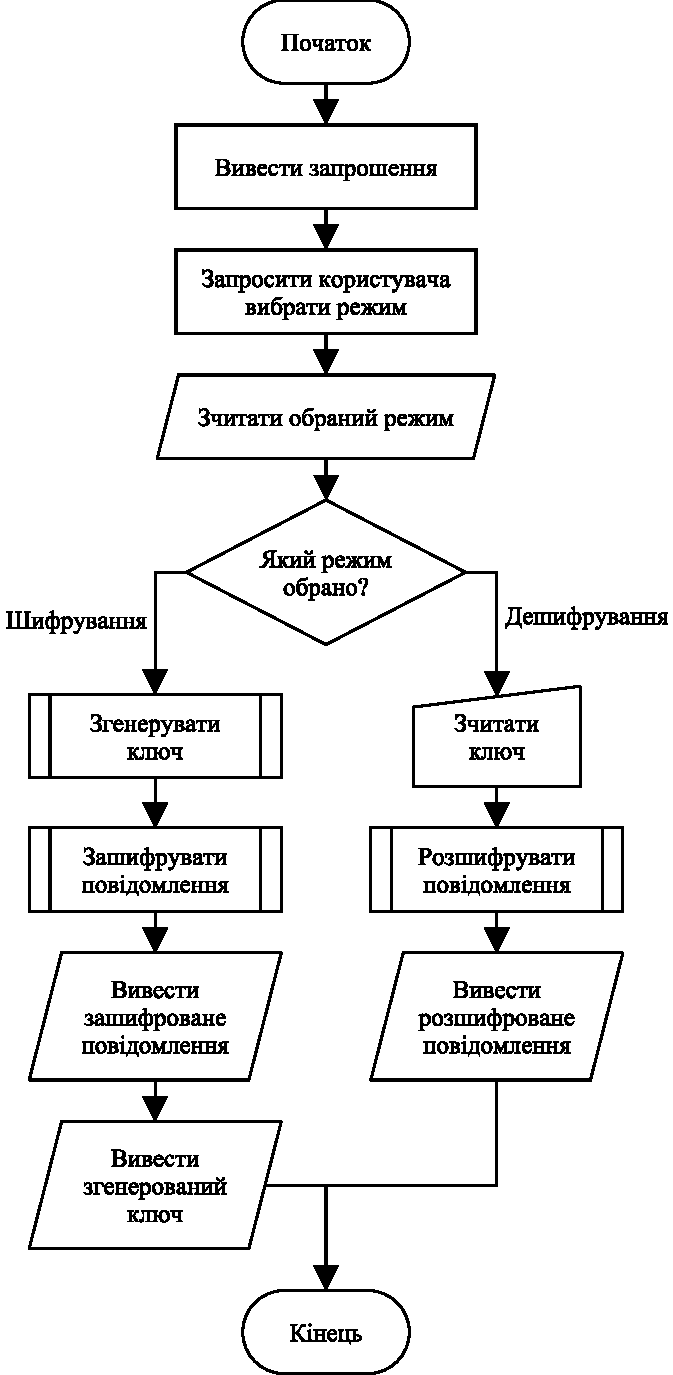
\includegraphics[scale=0.755]{diagrams/program-algorithm-flowchart.pdf}
				\caption{Блок-схема алгоритму роботи програми}
				\label{fig:programflowchart}
			\end{figure}
			\vspace*{\fill}
			\newpage
		\section{Блок-схема алгоритму шифрування}
			\vspace*{\fill}
			\begin{figure}[h]
				\centering
				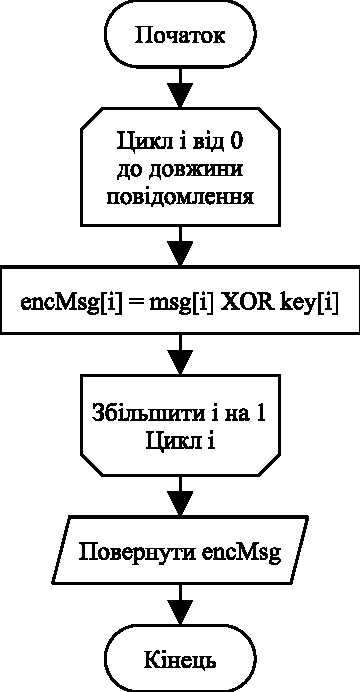
\includegraphics[scale=1]{diagrams/enciphering-algorithm-flowchart.pdf}
				\caption{Блок-схема алгоритму шифрування даних}
				\label{fig:encipheringflowchart}
			\end{figure}
			\vspace*{\fill}
			\newpage
		\section{Діаграма прецедентів}
			\vspace*{\fill}
			\begin{figure}[h]
				\centering
				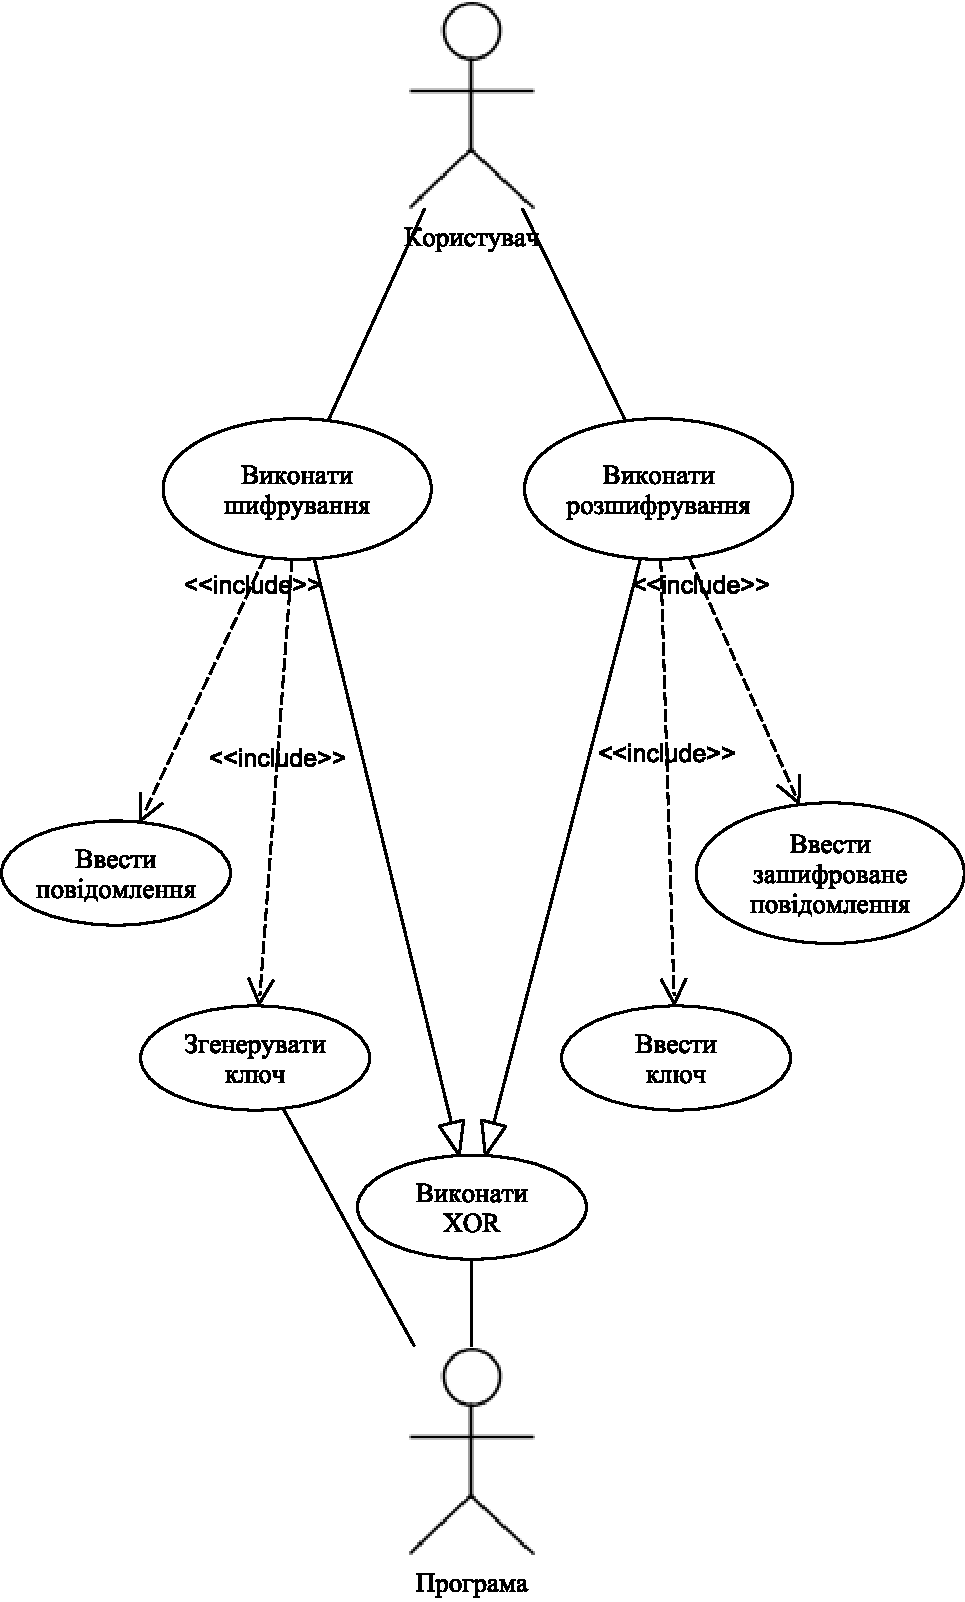
\includegraphics[scale=0.65]{diagrams/use-case-diag.pdf}
				\caption{Діаграма прецедентів при роботі з~користувачем}
				\label{fig:usecasediag}
			\end{figure}
			\vspace*{\fill}
		\section{Лістинг BlumBlumShub.hpp}
			\inputminted[tabsize=4,breaklines,breakbytokenanywhere,breaksymbol={},style=bw]{cpp}{source-codes/BlumBlumShub.hpp}
		\newpage
		\section{Лістинг BlumBlumShub.cpp}
			\inputminted[tabsize=4,breaklines,breakbytokenanywhere,breaksymbol={},style=bw]{cpp}{source-codes/BlumBlumShub.cpp}
		\newpage
		\section{Лістинг intpow.hpp}
			\inputminted[tabsize=4,breaklines,breakbytokenanywhere,breaksymbol={},style=bw]{cpp}{source-codes/intpow.h}
		\newpage
		\section{Лістинг intpow.cpp}
			\inputminted[tabsize=4,breaklines,breakbytokenanywhere,breaksymbol={},style=bw]{cpp}{source-codes/intpow.cpp}
		\newpage
		\section{Лістинг main.cpp}
			\inputminted[tabsize=4,breaklines,breakbytokenanywhere,breaksymbol={},style=bw]{cpp}{source-codes/main.cpp}
		\newpage
		%\section{Лістинг modulo.h}
		%	\inputminted{cpp}{source-codes/modulo.h}
		%\newpage
		\section{Лістинг msgmanip.hpp}
			\inputminted[tabsize=4,breaklines,breakbytokenanywhere,breaksymbol={},style=bw]{cpp}{source-codes/msgmanip.hpp}
		\newpage
		\section{Лістинг msgmanip.cpp}
			\inputminted[tabsize=4,breaklines,breakbytokenanywhere,breaksymbol={},style=bw]{cpp}{source-codes/msgmanip.cpp}
		\newpage
		
	\end{appendices}
\end{document}
